\section{Deep Learning Architectures \label{archi}}
    % Model descriptions
    \subsection{Deep Learning to Predict Molecular Weight from SMILES}
        \begin{itemize}
            \item The first model we will discuss is a DL model that receives an embedded SMILES string as input and as a result returns its prediction of the molecular weight. This model is shown in Fig.\ref{fig:mw-architecture}.
            \item Its architecture consisted first of a character embedding layer, that initially had random weights.
            \item This layer receives the pre-processed SMILES strings as input.
            \item Its output is then passed to a 1D Convolutional Neural Network (CNN) and is later flattened.
            \item This is followed with a fully connected layer that connects to a dropout layer.
            \item Finally, it ends with a 1 neuron dense layer that outputs the models prediction of the molecular weight.
            \item After the initial results seemed favorable the model was then tuned using the Talos Python library.
            \item Talos permitted us to run various models to see which combination of hyperparameters produced the best results.
            \item Some of the hyperparameters tuned were the batch size, number of units for the convolutional layers and fully connected layer, number of epochs, and the dropout rate for the dropout layer.
        \end{itemize}
    \subsection{Deep Learning to Predict XLogP from SMILES}
        \begin{itemize}
            \item The architecture for the second model was the same as the one used for predicting the molecular weight.
            \item In this case it also receives an embedded SMILES string as input, but it returns its prediction of the XLogP it should have.
        \end{itemize}
    \subsection{Deep Learning to Predict XLogP from SMILES and fragments}
        \begin{itemize}
            \item This model is similar to the first model, it differs in that it receives 2 inputs and has an embedding layer for each. 
            \item One of the embedding layers receives the SMILES strings and the other receives the RECAP fragments of the chemical compound.
            \item These two embedding layers are then concatenated and supplied to the 1D CNN as input.
            \item After this the architecture follows the same structure as the previous models.
            \item The output for this model was the predicted XLogP of the chemical compound.
        \end{itemize}
    
    % Figures
    \begin{figure}
        \centering
        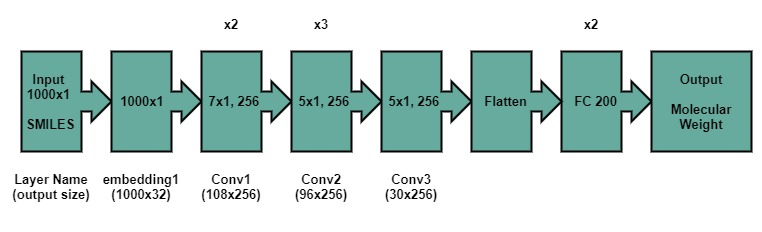
\includegraphics[width=0.5\textwidth]{figures/MW-model_arquitecture.jpg}
        \caption{The architecture of the model that predicts the molecular weight of a compound based on its SMILES string.}
        \label{fig:mw-architecture}
    \end{figure}
    \begin{figure}
        \centering
        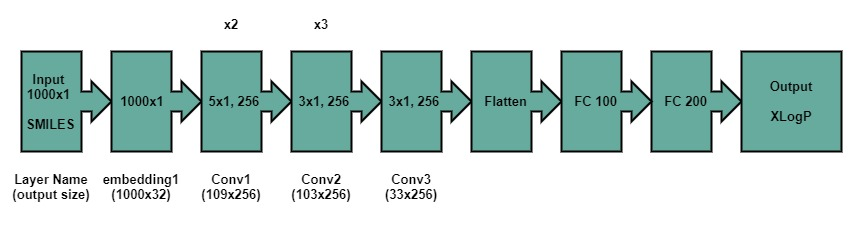
\includegraphics[width=0.5\textwidth]{figures/XLogP-model_arquitecture.jpg}
        \caption{The architecture of the model that predicts the XLogP of a compound based on its SMILES string.}
        \label{fig:xlogp-archi1}
    \end{figure}
    \begin{figure}
        \centering
        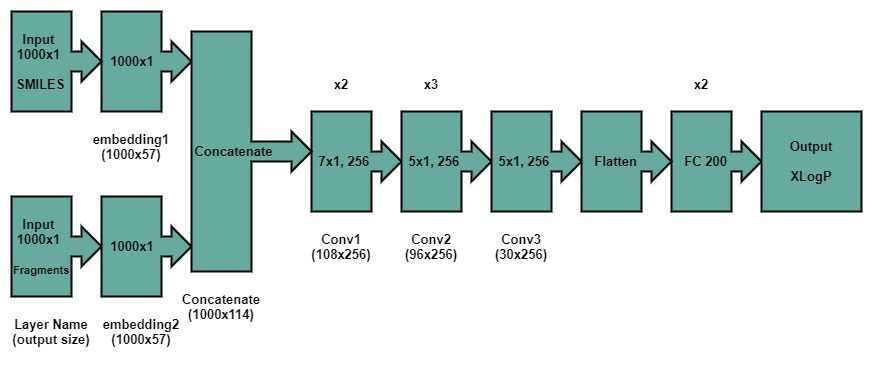
\includegraphics[width=0.5\textwidth]{figures/XLogP_frag_model_arquitecture.jpg}
        \caption{The architecture of the model that predicts the XLogP of a compound based on its SMILES string and RECAP fragments.}
        \label{fig:model23-mol-weight-loss}
    \end{figure}